\documentclass{beamer}

\usepackage[english]{babel}
\usepackage{graphicx}
\usepackage{caption}
\usepackage{hyperref}

\title{Individual variability of neural computations underlying flexible decisions}
\author{Hodivoianu Anamaria, Uceanu Alexandra, Gavrila Alexandru\\ University of Bucharest\\ Faculty of Mathematics and Informatics}
\date{\today}

\begin{document}

\begin{frame}
    \titlepage
\end{frame}

\begin{frame}{Study Overview}
    \begin{itemize}
        \item Better understanding of how the brain makes context-dependent decisions.
        \item Design an experiment with rats to study how they adapt their behavior based on task context.
        \item Key finding: Neural strategies vary across individuals, even when performing the same task successfully.
        \item Continuation of a similar study on monkeys: Context-dependent computation by recurrent dynamics in prefrontal cortex.
    \end{itemize}
\end{frame}

\begin{frame}{Context-Dependent Decision-Making}
    \begin{itemize}
        \item The ability to flexibly change responses based on context.
        \item Requires selecting and integrating relevant sensory evidence while ignoring irrelevant input.
    \end{itemize}
    \begin{minipage}{1\textwidth}
        \centering
        
\includegraphics[height=4cm]{decisions.jpg}
    \end{minipage}
\end{frame}

\begin{frame}{Why Monkeys and Rats?}
    Because they are \textbf{model organisms}. Model organisms are non-human species used to study biological processes that are conserved across species.\\
    \vspace{0.3cm}
    \textbf{Monkeys:}
    \begin{itemize}
        \item Closest analogs to human cognitive circuitry.
        \item Have a highly developed prefrontal cortex (PFC).
    \end{itemize}
    \vspace{0.2cm}
    \textbf{Rats:}
    \begin{itemize}
        \item Cost-effective, trainable, and widely used in neuroscience.
        \item Rats allowed precise, large-scale recordings of neural dynamics during context-dependent decisions.
    \end{itemize}
\end{frame}

\begin{frame}{Prefrontal Cortex in Monkeys and Rats}
    The PFC is the front part of the frontal lobe, responsible for high-level cognitive functions like planning, decision-making, and context switching.\\
    \vspace{0.4cm}
    \textbf{Monkeys:}
    \begin{itemize}
        \item \textbf{FEF} (frontal eye fields) – responsible for eye movements and motor planning.
    \end{itemize}
    \vspace{0.3cm}
    \textbf{Rats:}
    \begin{itemize}
        \item \textbf{FOF} (frontal orienting fields) – controls orienting responses and decision output.
    \end{itemize}
\end{frame}
    
\begin{frame}{Line Attractor: Concept \& Intuition}
    \begin{itemize}
        \item A stable trajectory in a neural dynamic system.
        \item Can only evolve along a 1D direction.
        \item Maintains its state when no new input is present.
        \item Decision making: brain accumulates evidence along a choice axis (line attractor).
    \end{itemize}
\end{frame}

\begin{frame}{Line Attractor: The Math Behind It}
    \begin{itemize}
        \item Neural activity in the brain evolves over time according to:
        \[
        \frac{d\vec{r}}{dt} = M \vec{r}
        \]
        \item \( \vec{r} \): vector of neural activity (system state)  
        \( M \): dynamics matrix (how activity evolves)
        \item To understand this system, we look at its:
        \begin{itemize}
            \item \textbf{Eigenvectors} – directions the system moves in
            \item \textbf{Eigenvalues} – how fast it moves or decays along those directions
        \end{itemize}
        \item A \textbf{line attractor} appears when:
        \begin{itemize}
            \item One eigenvalue = 0 → system is stable along that direction (no decay)
            \item All other eigenvalues \( < 0 \) → other directions fade over time
        \end{itemize}
        \item Result: the system stays on a line in neural space and accumulates input there → \textbf{decision axis}
    \end{itemize}
\end{frame}

\begin{frame}{Selection Vector}
    \[
    \Delta \text{choice} = \vec{s} \cdot \vec{i}
    \]
    \begin{itemize}
        \item The brain receives input from many sources (motion, color, etc.).
        \item The \textbf{selection vector} \( \vec{s} \) tells the system which input to care about.
        \item The input \( \vec{i} \) is a pulse (e.g., motion or color).
        \item The dot product \( \vec{s} \cdot \vec{i} \) decides how much that input moves the system along the decision line (line attractor).
    \end{itemize}
\end{frame}

\begin{frame}{The Monkey Study (Mante et al., 2013)}
    \begin{itemize}
        \item Task: motion vs color, cued by context.
        \item Inputs from both dimensions entered PFC.
        \item Explained by: \textbf{line attractor} + \textbf{selection vector}.
    \end{itemize}
    \begin{minipage}{1\textwidth}
        \centering
        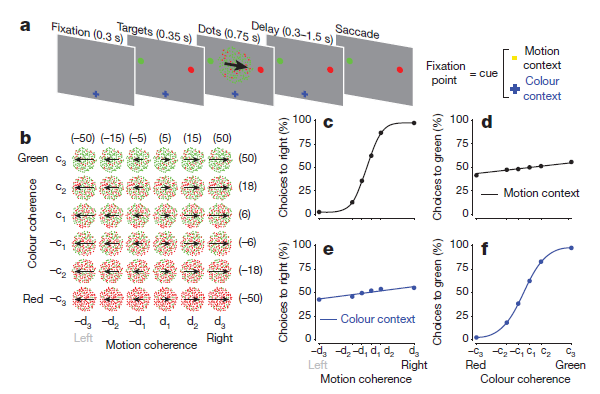
\includegraphics[height=6cm]{monkey_experiment.png}
    \end{minipage}
\end{frame}

\begin{frame}{Recurrent Neural Networks (RNNs) in the Monkey Study}
    \begin{itemize}
        \item Trained RNNs to replicate the monkey's task.
        \item RNNs received streams of motion and color input and a context cue.
        \item The trained RNNs:
        \begin{itemize}
            \item Learned to integrate only the relevant input (motion or color) based on context.
            \item Developed internal dynamics with a \textbf{line attractor} and context-specific \textbf{selection vectors}.
        \end{itemize}
    \end{itemize}
\end{frame}

\begin{frame}
\frametitle{Rat Task}

Rats solve a context-dependent task
\begin{figure}[h!]
   	\centering
   	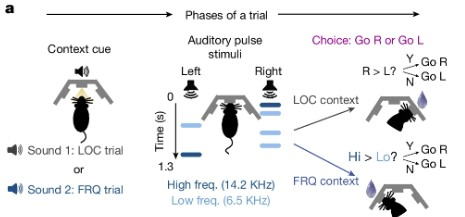
\includegraphics[width=\textwidth]{design.jpg}
   	\caption{Experiment Design}
   	\label{fig:design}
\end{figure}
\end{frame}

\begin{frame}
\frametitle{Frontal Orienting Fields}
Measuring neural activity in FOF:

\begin{itemize}
	\item Irrelevant information is not gated out
	\item Same choice axis in both contexts
	\item Similar results in monkeys
\end{itemize}

\begin{figure}[h!]
	\centering
	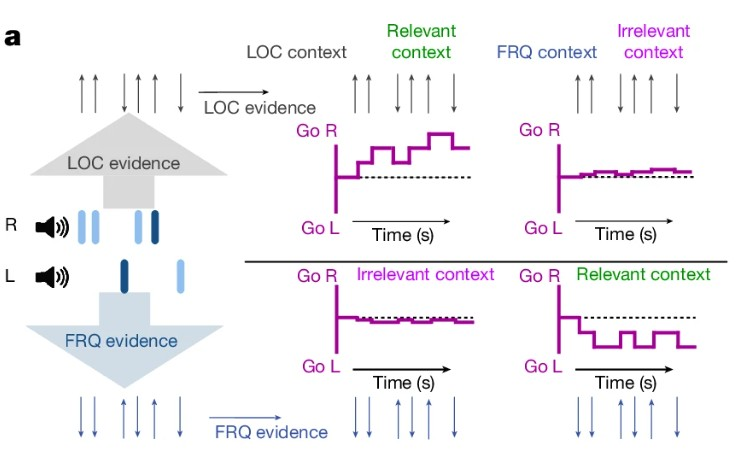
\includegraphics[width=0.75\textwidth]{impact.jpg}
	\caption{Pulses of Evidence Have Greater Influence When Relevant}
    \label{fig:impact}
\end{figure}
\end{frame}

\begin{frame}
\frametitle{Theorethical Framework}
How is the impact of a pulse of evidence controlled?

Hypothesis: Choice axis = Line attractor

Implication: Change in position along the choice axis = $s \cdot i$

Condition: The product should be greater in the relevant context

Across contexts:

\begin{itemize}
	\item Modify input vector $i$
	\item Modify selection vector $s$
\end{itemize}
\end{frame}

\begin{frame}
\frametitle{Three Components(1)}
DIM (direct input modulation) - change in input vector parallel to choice axis, immediate difference across contexts

\begin{figure}[h!]
	\centering
	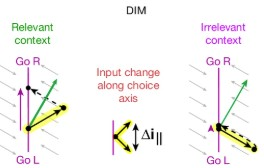
\includegraphics[width=0.7\textwidth]{dim.jpg}
	\caption{DIM \\ Pink - Choice Axis, Green - Selection Vector, Black - Input Vector}
    \label{fig:dim}
\end{figure}
\end{frame}

\begin{frame}
\frametitle{Three Components(2)}
IIM (indirect input modulation) - change in input vector orthogonal to choice axis, gradual difference across contexts

\begin{figure}[h!]
	\centering
	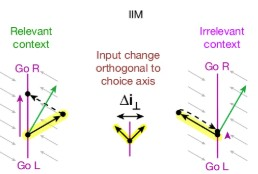
\includegraphics[width=0.7\textwidth]{iim.jpg}
	\caption{IIM}
    \label{fig:iim}
\end{figure}
\end{frame}

\begin{frame}
\frametitle{Three Components(3)}
SVM (selection vector modulation) - recurrent dynamics change to adjust to relevant/ irrelevant information, gradual difference across contexts

\begin{figure}[h!]
	\centering
	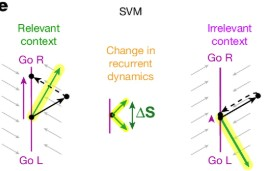
\includegraphics[width=0.7\textwidth]{svm.jpg}
	\caption{SVM}
    \label{fig:svm}
\end{figure}
\end{frame}

\begin{frame}
\frametitle{Variability}

\begin{itemize}
	\item All combinations are possible
	\item Theory matched experimental data
	\item Rats used different combinations of DIM, IIM, SVM
	\item All lead to good performance
\end{itemize}
\begin{figure}[h!]
	\centering
	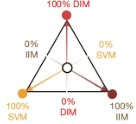
\includegraphics[width=0.4\textwidth]{triangle.jpg}
	\caption{Space of Networks that Can Solve the Task Larger than Previously Thought}
    \label{fig:triangle}
\end{figure}
\end{frame}

\begin{frame}
\frametitle{Biological Implications}
Pulse effect:
\begin{itemize}
	\item DIM: immediate
	\item IIM \& SVM: changes with time (last pulse may have less influence)
\end{itemize}

Context-dependence handling:
\begin{itemize}
	\item SVM: in decision-making regions
	\item DIM \& IIM: outside decision-making regions, probably in:
		\begin{itemize}
			\item sensory regions
			\item pathways from sensory to decision-making regions
		\end{itemize} 
\end{itemize}
\end{frame}

\begin{frame}{Pulse Analyses Distinguish Solutions}
    \begin{itemize}
        \item Artificial model networks can be used to illustrate approaches to solving the task
        \begin{itemize}
            \item Mante et al. in the monkey study developed an RNN and trained it
            \item They observed important similarities in the experimental data and the trained RNNs
            \item Upon further analysis the researchers found SVM as the leading candidate used in decision-making.
        \end{itemize}
        \item Fast vs slow separation along the choice axis (immediate = DIM; delayed = IIM/SVM)
    \end{itemize}
\end{frame}

\begin{frame}{Introduction to RNNs}

\begin{itemize}
    \item What are RNNs?
    \item How do they work?
    \item Why use them?
\end{itemize}
    
\end{frame}

\begin{frame}{Introduction to Recurrent Neural Networks(2)}

\centering
\begin{minipage}{0.48\linewidth}
    \centering
    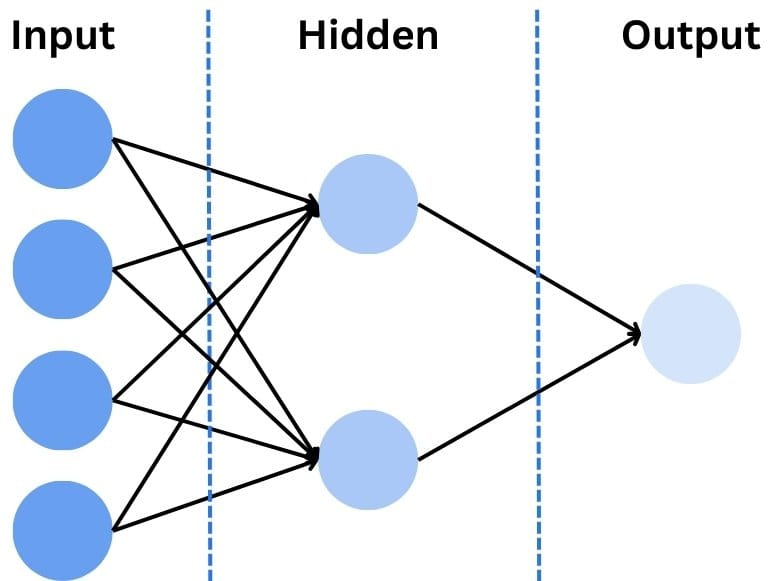
\includegraphics[width=\linewidth]{classical-neural-network.jpg}
    \label{fig:cnn}
    {\tiny Source: \href{https://www.simplyblock.io/blog/image-recognition-with-neural-networks/}{SimplyBlock}}
\end{minipage}
\hfill
\begin{minipage}{0.48\linewidth}
    \centering
    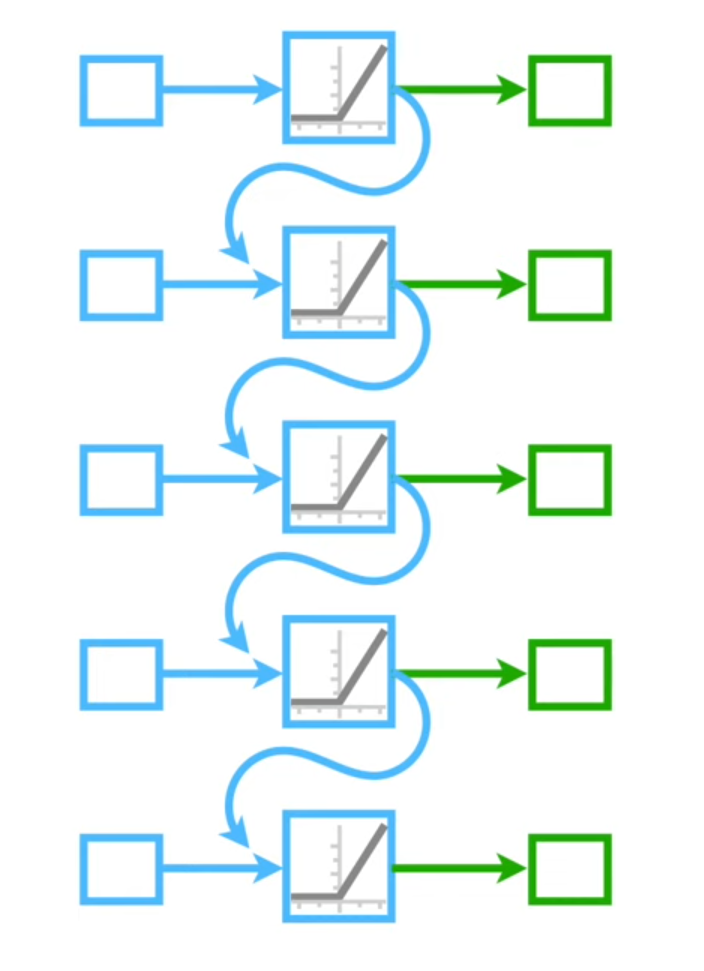
\includegraphics[width=\linewidth]{RNN.png}
    \label{fig:rnn}
    {\tiny Source: \href{https://www.youtube.com/watch?v=AsNTP8Kwu80}{StatQuest}}
\end{minipage}
    
\end{frame}

\begin{frame}{New Observation in Linearization}
    \begin{itemize}
        \item In the current study, Pagan et al. found that the results from Mante's study were biased because of the linearization used
        \item Activation-space hides input modulations because it linearizes before nonlinearity.
        \item Firing-rate-space linearizes after nonlinearity, revealing all three components.
    \end{itemize}
\end{frame}

\begin{frame}{RNN Training vs Engineering}

    \begin{itemize}
        \item Trained many RNNs on the same rat task
        \begin{itemize}
            \item Backpropagation-through-time (BPTT)
            \begin{itemize}
                \item Sends trained RNNs to SVM corner
            \end{itemize}
            \item Engineered RNNs
            \begin{itemize}
                \item Analytical construction via derived constraints
            \end{itemize}
        \end{itemize}
    \end{itemize}
    
\end{frame}

\begin{frame}{RNN Training vs Engineering(2)}
    \begin{figure}
        \centering
        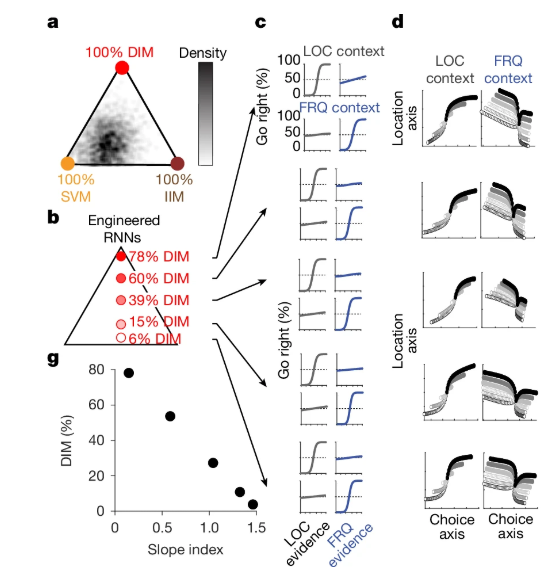
\includegraphics[width=0.5\linewidth]{rnn-cluster.png}
        \caption{RNN Training Dispersion}
        \label{fig:rnn-training}
    \end{figure}
\end{frame}

\begin{frame}{Engineered RNNs}
    \begin{itemize}
        \item Started by analyzing standard trained RNNs to understand their internal dynamics
        \item Derived mathematical equations that characterize how input and recurrent weights contribute to each component (DIM, IIM, SVM)
        \item Used these equations to construct new RNNs from scratch that lie at any desired point in the solution triangle
    \end{itemize}
\end{frame}

\begin{frame}{Linking Neural and Behaviour Variability}
    \begin{itemize}
        \item Study based on relative weight that evidence presented across different time points of a trial has on the subject's choices
        \item If that is correct, then fast vs slow context-dependent effects on the choice axis should have corresponding behavioural correlates
        \item Tested the prediction on RNNs engineered to solve the task using different amounts of DIM.
        \item The RNNs data was tightly linked with rats experimental data.
    \end{itemize}
\end{frame}

\begin{frame}{Conclusion}
    \begin{itemize}
        \item Individual variability arises from different mixes of DIM, IIM, SVM
        \item Neural differential pulse responses predict behavioral weighting of early vs late evidence
        \item Broader insight
    \end{itemize}
\end{frame}

\begin{frame}
  \centering
  \Huge{Thank You!}
\end{frame}

\end{document}



























